\begin{center}
   {\colorbox{grey2}{
         \begin{minipage}[t]{0.9\textwidth}
\subsubsection*{Scope}
This Pirana Quick Guide explains how add NONMEM (nmfe) installations
to Pirana. This procedure is not required for PsN installations, which
are automatically recognized if PsN is configured appropriately. It
will also be discussed how to set up installations that use Intel
Fortran v11 as compiler within Pirana. Note: in this quick guide it
will be assumed that you already have installed NONMEM.
          \end{minipage}
      }
   }
\end{center}

\subsubsection*{Add NONMEM installation setting window}
\begin{itemize}
\item Go to File $\rightarrow$ Settings $\rightarrow$ NONMEM. The
  dialog window shown in Figure 1 appears.
\item In this dialo, local (top part) and remote (bottom part) NONMEM
  installations may be defined.
\end{itemize}

\begin{figure}[h] \centering
    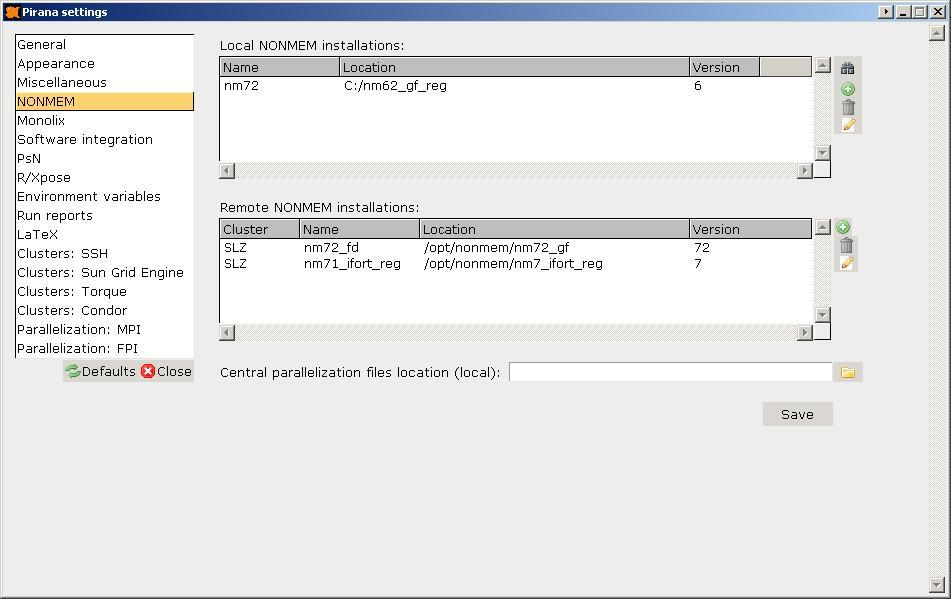
\includegraphics[scale=.42]{images/addnonmem_1.jpg}
    \caption{Adding a NONMEM installation\label{fig:Fig1}}
\end{figure}

\subsubsection*{Adding local nonmem installations }
\begin{itemize}
\item By pressing the Find icon (Figure \ref{fig:Fig1}, blue square), Pirana will
  automatically attempt to find any local NONMEM installations at
  common installation locations.
\item If you installed NONMEM at a non-standard location and Pirana is
  not able to find it automatically, you will have to add it manually, by
  pressing the \emph{\Large{+}} button (Figure \ref{fig:Fig1}, red square).
\item A window (Figure \ref{fig:Fig2}) will appear where the name and location of
  the NONMEM installation may be entered. The version of NONMEM will
  be automatically detected.
\item After adding NONMEM installations, please press the Save button (Figure
  \ref{fig:Fig1}). The local NONMEM installations will then be available in Pirana.
\end{itemize}

\begin{figure}[h] \centering
    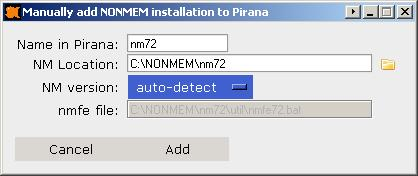
\includegraphics[scale=.5]{images/addnonmem_2.jpg}
    \caption{Adding a local NONMEM installation\label{fig:Fig2}}
\end{figure}

\subsubsection*{Adding remote nonmem installations }
\begin{itemize}
\item Auto-detection of NONMEM installations is not available for
  remote NONMEM installations, they will have to be added manually.
\item Press the \emph{\Large{+}} button next to \emph{Remote NONMEM}
  installations, to add a remote installation.
\item A window (Figure \ref{fig:Fig3}) appears, in which the installation name, the
  associated cluster, the location and the version can be defined.
\item After adding NONMEM installations, press the Save button (Figure
  \ref{fig:Fig1}). The remote NONMEM installations are now available in Pirana.
\end{itemize}

\begin{figure}[h] \centering
    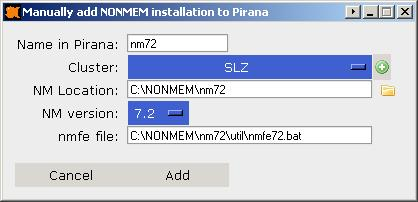
\includegraphics[scale=.5]{images/addnonmem_3.jpg}
    \caption{Adding a remote NONMEM installation\label{fig:Fig3}}
\end{figure}

\subsubsection*{Using Intel Fortran 11 for Windows together with NONMEM/PsN}
The Intel Fortran 11 compiler requires the user to set several
environmental variables. If these variables are correctly defined
system-wide, NONMEM installations using Intel Fortran should already
work. However, if you are not able to set the environment variables
system-wide, or you experience problems, you can also use Pirana to
set them for you.

\begin{itemize}
\item Please refer to posts on NMusers (such as
  \href{'http://www.cognigencorp.com/nonmem/current/2009-October/2077.html''}{this}
  one) where it is explained how environmental variables should be
  defined for Intel Fortran. These may differ slightly from system to
  system, so we can't give a fixed solution here. The common way in
  Windows to set these environment variables is by going to the
  Control panel $\rightarrow$ System settings $\rightarrow$
  Environment variables.  However, Pirana offers three alternative
  solutions to define the required environmental variables.
\item The first option is through Tools $\rightarrow$ NONMEM
  $\rightarrow$ Environmental variables. Setting the environment
  variables here will set them prior to executing a model (nmfe-only).
\item The second option is through File $\rightarrow$ Settings
  $\rightarrow$ Software integration $\rightarrow$ 'Add this to path
  at Pirana startup. Note that this only adds locations to the PATH
  environment variable. Most likely, you will have to set a few more
  environment variables as well.
\item The last option is by adding a text file add\_env.txt or
  set\_env.txt to the main Pirana folder. These text files can be used
  to \emph{add} to or \emph{set} any environmental variables. These
  files could for instance look as below.
\end{itemize}
   {\colorbox{grey2}{
         \begin{minipage}[t]{0.5\textwidth}
          {\ttfamily
   PATH=C:$\backslash$nmvi$\backslash$run;C:$\backslash$MinGW$\backslash$bin\\
   LIB=C:$\backslash$Program files$\backslash$Intel
   fortran$\backslash$bin
}
          \end{minipage}
      }
   }

